\chapter{Конструкторский раздел}
\label{cha:design}

\section{Разработка алгоритма}
Рассмотренный алгоритм GSP в основном используется в торговли, и обычно под транзакцией имеется ввиду покупка определенного набора товаров (продуктов, книг и т.д.). В случае анализа активности пользователей САПР, зачастую, данные представлены в виде последовательности команд с параметрами. Кроме этого, данный алгоритм учитывает кто совершил покупку, то есть id клиента.
Поэтому за одну транзакцию примем выполнение одной команды, а за id клиента - id сессии. В таком случае поддержкой последовательности команд будет отношение числа сессий поддерживающих данную последовательность к общему их количеству. 

\section{Особенности предлагаемого метода}
%На вход разрабатываемому алгоритму будет подаваться минимальный уровень поддержки, минимальный и максимальный разрывы между командами и таблица базы данных команд со следующими полями:
%На вход программе подаются таблица базы данных команд, минимальный уровень поддержки, минимальный и максимальный разрывы между командами.
Обычно логи представлены в текстовом виде, поэтому перед обработкой их алгоритмом, данные будут преобразовываться в таблицу базы данных со следующими полями:
\begin{itemize}
	\item[---] id; %выполненной команды
	\item[---] id сессии в течение которой была исполнена команда;
	\item[---] время в которое команда была выполнена;
	\item[---] имя команды.
\end{itemize}

В алгоритме GSP элемент последовательности может содержать несколько транзакций, если они были совершены в пределах заданного скользящего окна. Кроме этого, в одну транзакцию может входить несколько предметов. В таком случае не учитывается в каком порядке были приобретены продукты в пределах одной транзакции. Данный подход пригоден для использования в области торговли, но в случае анализа активности пользователей,
все действия выполняются в определенной последовательности и
%необходимо учитывать их порядок.
учитывание порядка каждого из них даст больше информации в результате.
%в большинстве случаев, для каждого выполненого действия можно определить его порядок -- перед и после какого действия оно было совершено.
Поэтому для разрабатываемого метода элемент последовательности может состоять только из одной транзакции, в которую будет входить только одна команда. Следовательно, нет необходимости в использовании скользящего окна в пределах которого, совершенные транзакции считаются совершенными одновременно. Но в таком случае возникает проблема с определением порядка выполнения команд выполненных в один момент времени. Чтобы ее решить, будем считать, что команды выполнились в том порядке, в котором они были записаны в лог.

%Также, стоит отметить, что элемент последовательности в разрабатываемом методе может состоять только из одной транзакции, в отличии от алгоритма GSP, где он может содержать несколько транзакций. Поэтому нет необходимости в использовании скользящего окна в пределах которого, совершенные транзакции считаются совершенными одновременно. В таком случае возникает проблема с определением порядка выполнения команд выполненных в один момент времени. Чтобы ее решить, будем считать, что команды выполнились в том порядке, в котором они были записаны в лог.

\section{Ключевые этапы алгоритма}
Как и в алогритме GSP, разрабатываемый метод будет состоять из двух основных этапов:

\begin{enumerate}
	\item[1.] Генерация кандидатов.
	\item[2.] Подсчет поддержки кандидатов.
\end{enumerate}

%Но их реализация будет отличаться от первоначальной

\subsection{Генерация кандидатов}

Данный этап описывает как генерируются последовательности-кандидаты перед проверкой их уровня поддержки. Нужно сгенерировать всех возможных кандидатов, стараясь свести их количество к минимуму.

Как было описано выше, в алгоритме GSP данный этап состоит из двух частей: объединение и упрощение. Но по-скольку в нашем случае каждый элемент последовательности может состоять только из одной транзакции, отпадает необходимость в упрощении. Также, стоит отметить, что на первом шаге алгоритма в качестве кандидатов нужно просто взять всевозможные одно-элементные последовательности.

На рисунке \ref{generateCandidates} представлена блок-схема данного этапа.

%\subsection{Подсчет поддержки кандидатов}
%
%После получения списка кандидатов, нужно определить какие последовательности удовлетворяют заданному минимальному уровню поддержки, а какие нет. Для этого необходимо для каждого кандидата определить кол-во сессий поддерживающих его. На рисунке \ref{sessionSupportsSequence} приведена схема проверки поддержки кандидата сессией.

\newpage
\begin{figure}[h!]
	\centering
	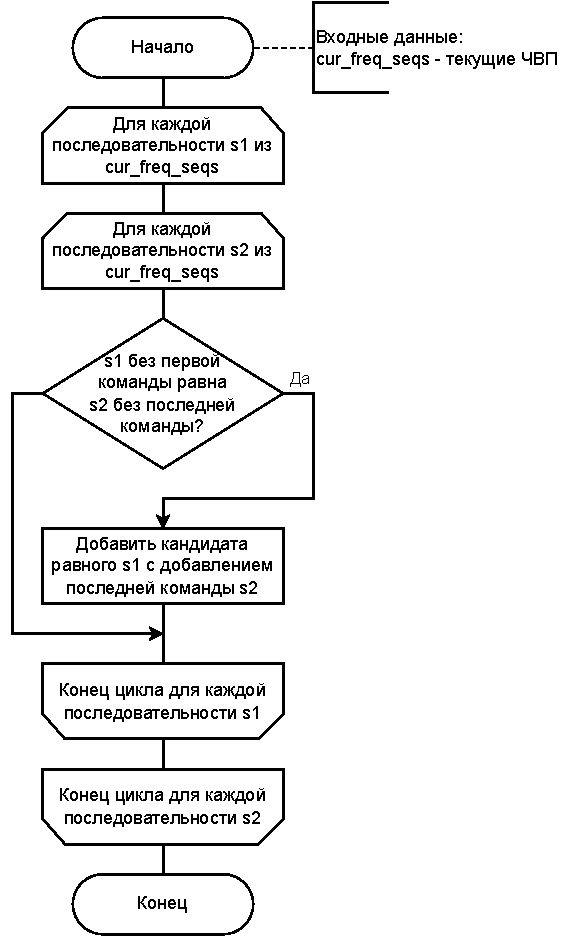
\includegraphics[width=0.8\textwidth]{inc/img/generateCandidates.drawio.pdf}
	\caption{Генерация кандидатов}
	\label{generateCandidates}
\end{figure}

%\begin{figure}[h!]
%	\centering
%	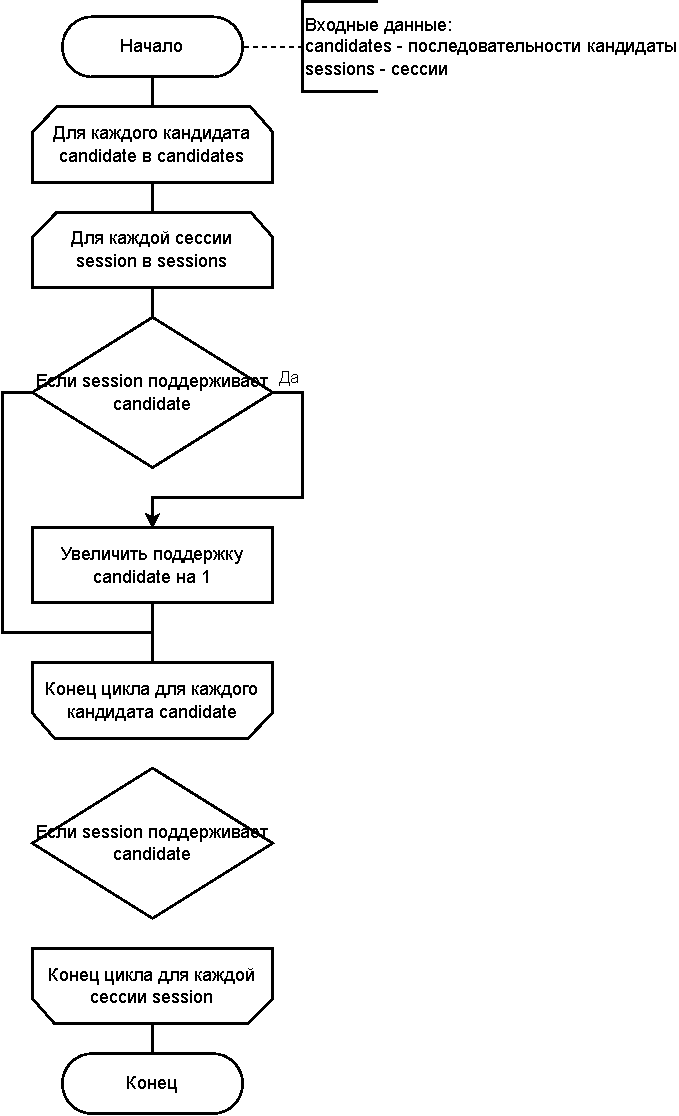
\includegraphics[width=0.8\textwidth]{inc/img/countSupport.drawio.pdf}
%	\caption{Подсчет поддержки кандидатов}
%	\label{countSupport}
%\end{figure}

\newpage
\subsection{Подсчет поддержки кандидатов}

После получения списка кандидатов, нужно определить какие последовательности удовлетворяют заданному минимальному уровню поддержки, а какие нет. Для этого необходимо для каждого кандидата определить кол-во сессий поддерживающих его. На рисунках \ref{sessionSupportsSequence}-\ref{backward_phase} приведена схема проверки поддержки кандидата сессией.

%\newpage
%\begin{figure}[h!]
%	\centering
%	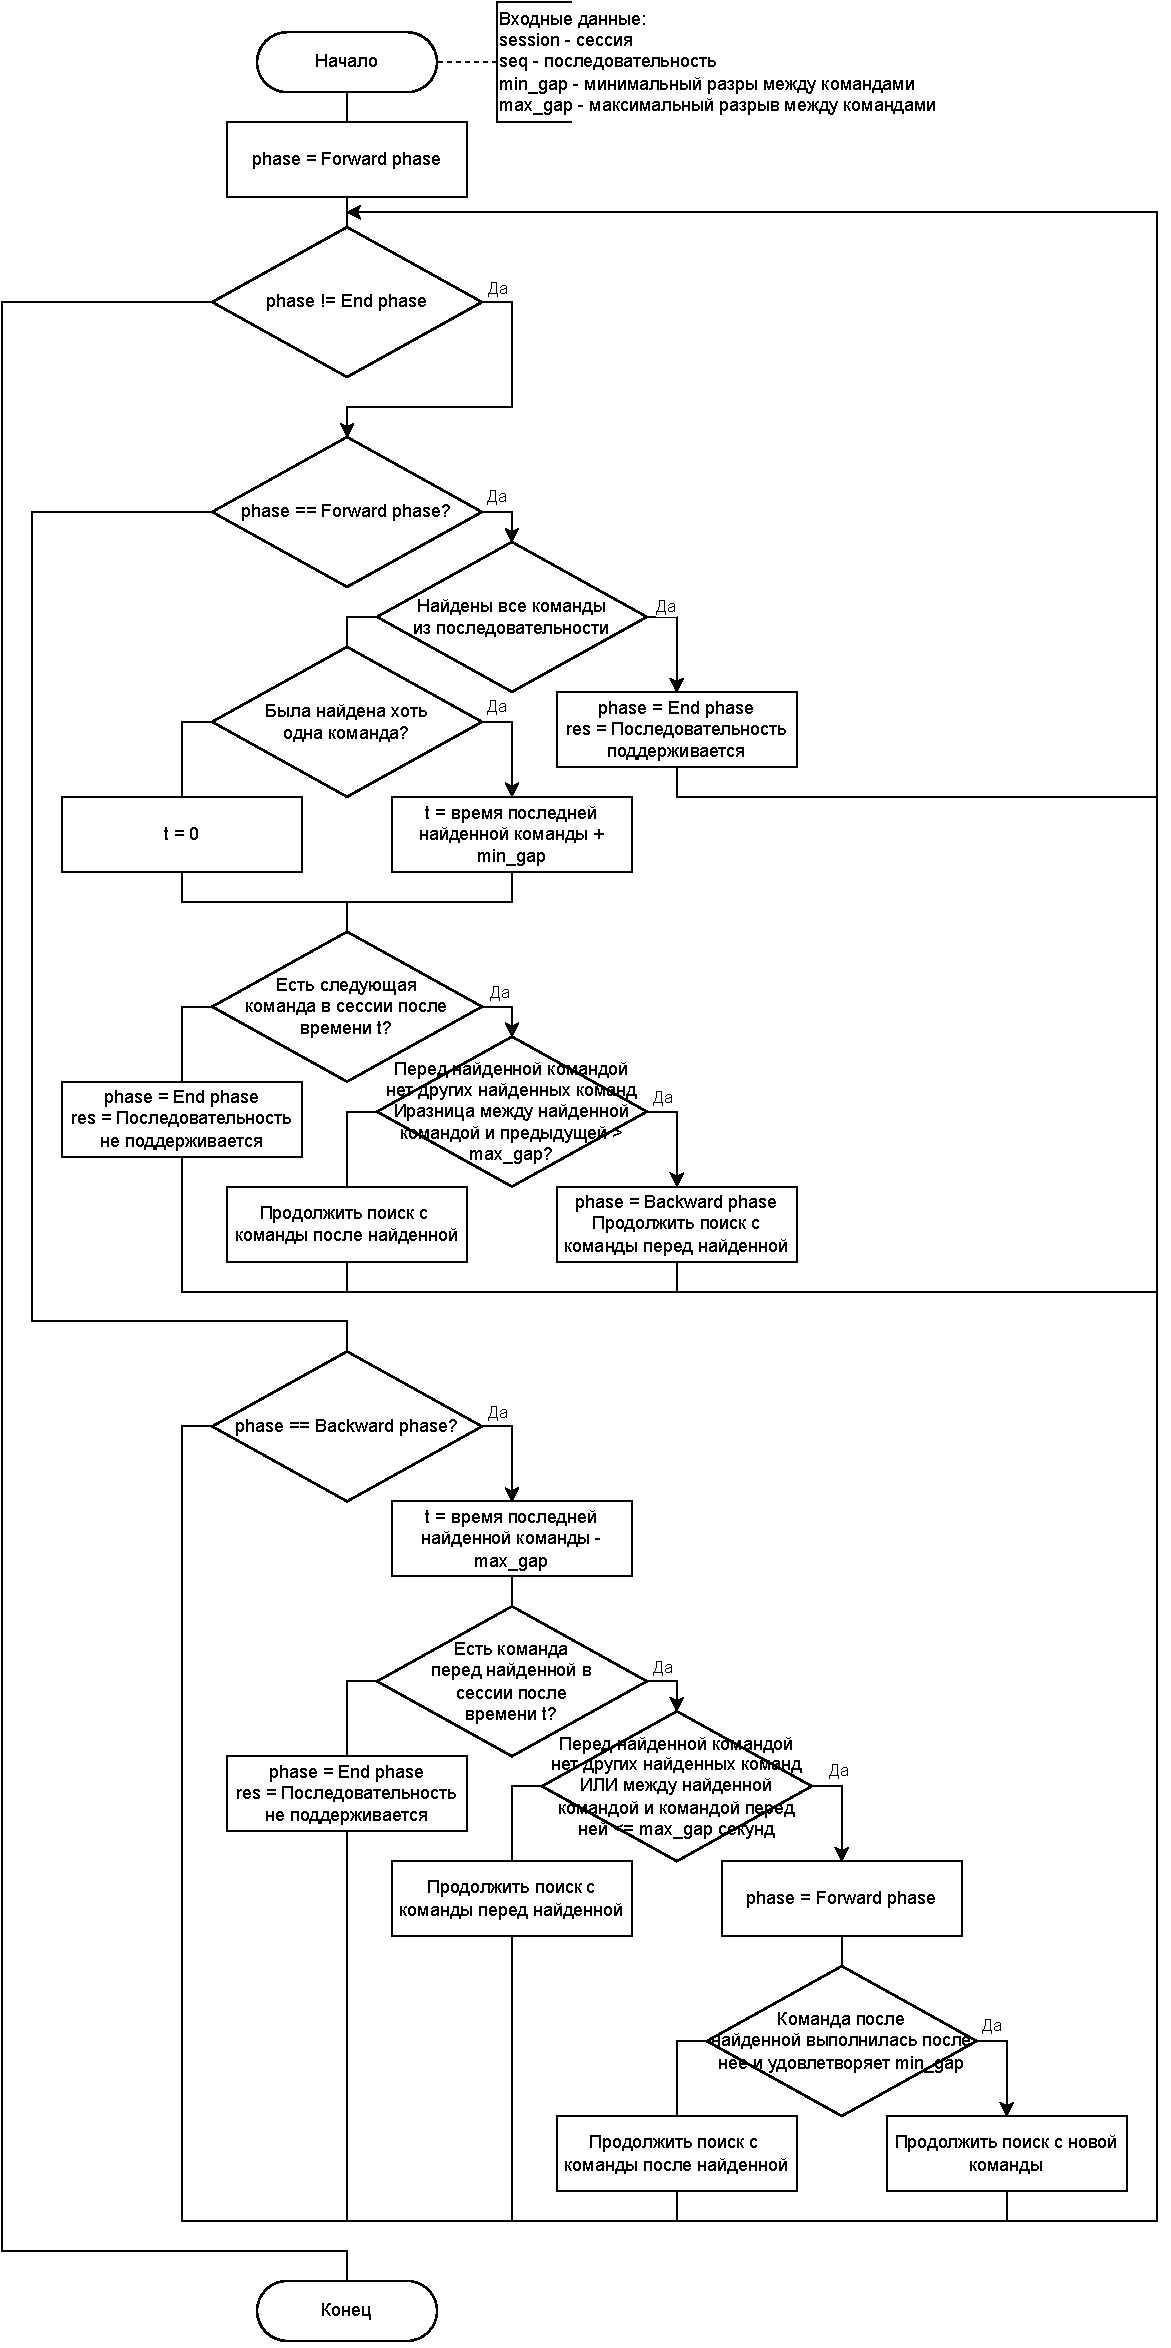
\includegraphics[width=0.7\textwidth]{inc/img/sessionSupportsSequence.drawio.pdf}
%	\caption{Проверка поддержки кандидата сессией}
%	\label{sessionSupportsSequence}
%\end{figure}

\begin{figure}[h!]
	\centering
	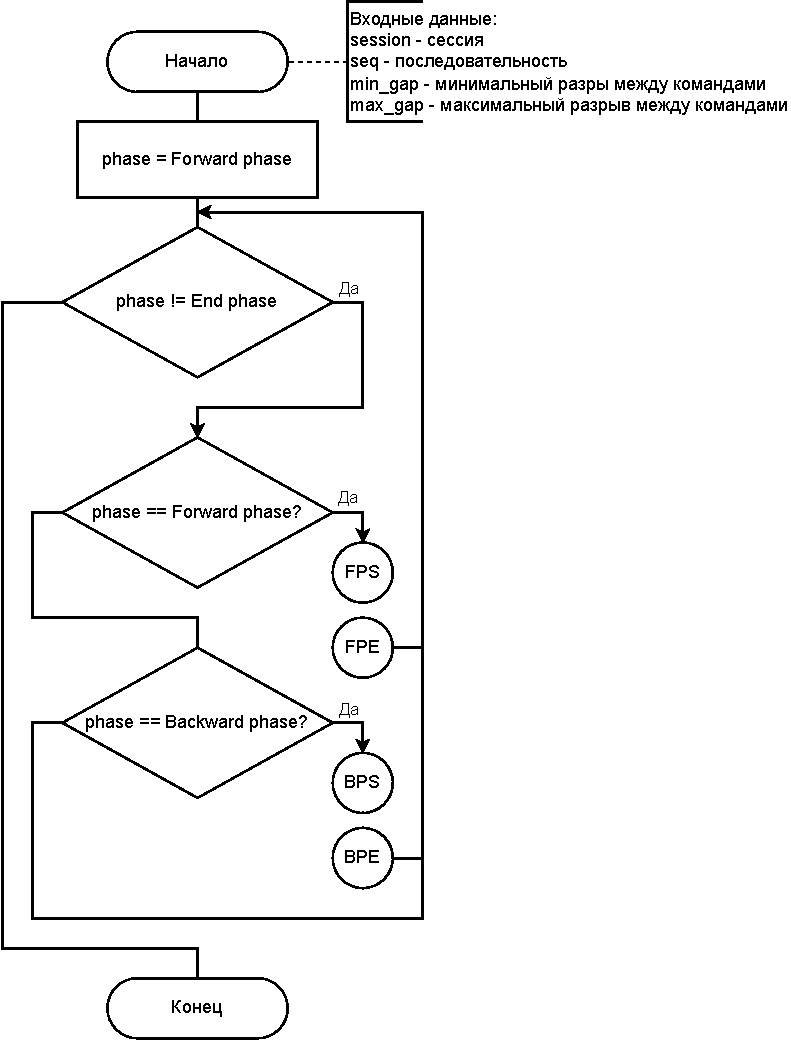
\includegraphics[width=0.65\textwidth]{inc/img/sessionSupportsSequence2.drawio.pdf}
	\caption{Проверка поддержки кандидата сессией, часть 1}
	\label{sessionSupportsSequence}
\end{figure}

\newpage
\begin{figure}[h!]
	\centering
	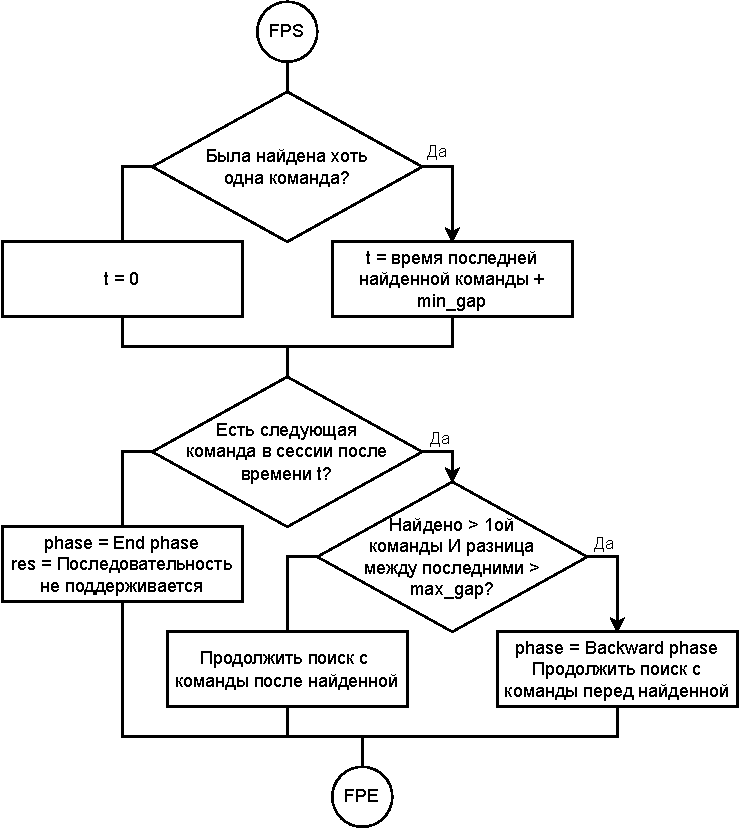
\includegraphics[width=1\textwidth]{inc/img/forward_phase.drawio.pdf}
	\caption{Проверка поддержки кандидата сессией, часть 2}
	\label{forward_phase}
\end{figure}

\newpage
\begin{figure}[h!]
	\centering
	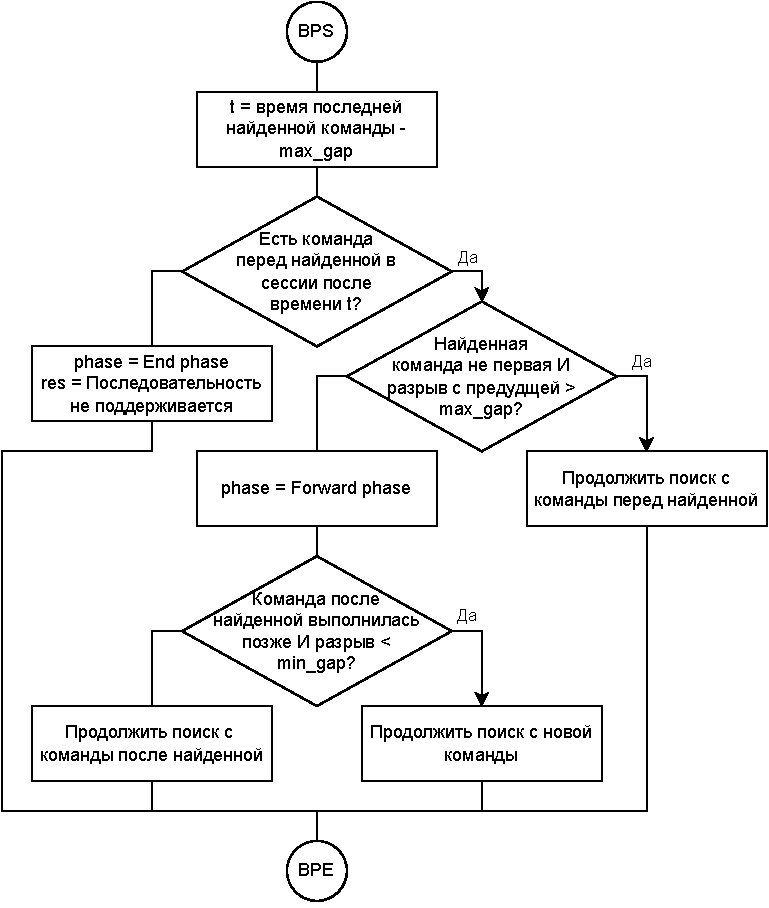
\includegraphics[width=1\textwidth]{inc/img/backward_phase.drawio.pdf}
	\caption{Проверка поддержки кандидата сессией, часть 3}
	\label{backward_phase}
\end{figure}

\newpage
\section{Используемые структуры данных}
Для работы алгоритма необходимо описать структуры данных для следующих основных объектов:
\begin{enumerate}
	\item[---] транзакция (команда);
	\item[---] последовательность;
	\item[---] сессия.
\end{enumerate}

Для транзакции (команды), в соответствии с таблицей базы данных подающейся на вход алгоритму, выделены следующие параметры:
id, id сессии в течение которой была исполнена команда, время в которое команда была выполнена, имя команды.
%\begin{itemize}
%	\item[---] id; %выполненной команды
%	\item[---] id сессии в течение которой была исполнена команда;
%	\item[---] время в которое команда была выполнена;
%	\item[---] имя команды.
%\end{itemize}

Последовательность будет хранить массив команд, собственное значение поддержки и другие характеристики, относящиеся непосредственно к последовательности. %lift

Для сессии можно выделить следующие поля:
id, массив команд, альтернативное представление сессии в виде массива односвязных списков хранящих время выполнения команд.
%\begin{itemize}
%	\item[---] id; %сессии
%	\item[---] массив команд;
%	\item[---] альтернативное представление сессии в виде массива односвязных списков хранящих время выполнения команд.
%\end{itemize}
Последнее поле сессии используется для подсчета поддержки кандидатов. 

%\begin{table}[H]
%	\begin{center}
%		\caption{Пример сессии}
%		\label{session_example}
%		""\newline
%		\begin{tabular}{ | c | c | }
%			\hline
%			Время транзакции & Команда \\ \hline
%			1 & 2 \\ \hline
%			1 & 2 \\ \hline
%			5 & 2 \\ \hline
%			8 & 3 \\ \hline
%			8 & 4 \\ \hline
%		\end{tabular}
%	\end{center}
%\end{table}
%
%\begin{table}[H]
%	\begin{center}
%		\caption{Альтернативное представление}
%		\label{session_alternative_representation}
%		""\newline
%		\begin{tabular}{ | c | c | }
%			\hline
%			Команда & Времена \\ \hline
%			1 & $\rightarrow$ NULL \\ \hline
%			2 & $\rightarrow 1 \rightarrow 1 \rightarrow 5 \rightarrow$ NULL \\ \hline
%			3 & $\rightarrow 8 \rightarrow$ NULL \\ \hline
%			4 & $\rightarrow 8 \rightarrow$ NULL \\ \hline
%		\end{tabular}
%	\end{center}
%\end{table}

\begin{table}[H]
	\begin{minipage}[h]{0.49\linewidth}
		\caption{Пример сессии}
		\label{session_example}
		""\newline
		\begin{tabular}{ | c | c | }
			\hline
			Время транзакции & Команда \\ \hline
			1 & 2 \\ \hline
			1 & 2 \\ \hline
			5 & 2 \\ \hline
			8 & 3 \\ \hline
			8 & 4 \\ \hline
		\end{tabular}
	\end{minipage}
	\begin{minipage}[h]{0.49\linewidth}
		\caption{Альтернативное представление сессии}
		\label{session_alternative_representation}
		""\newline
		\begin{tabular}{ | c | c | }
			\hline
			Команда & Времена \\ \hline
			1 & $\rightarrow$ NULL \\ \hline
			2 & $\rightarrow 1 \rightarrow 1 \rightarrow 5 \rightarrow$ NULL \\ \hline
			3 & $\rightarrow 8 \rightarrow$ NULL \\ \hline
			4 & $\rightarrow 8 \rightarrow$ NULL \\ \hline
		\end{tabular}
	\end{minipage}
\end{table}


\textbf{Пример проверки поддержки последовательности сессией.} Допустим есть сессия (таблицы \ref{session_example}-\ref{session_alternative_representation}) и нам нужно определить поддерживает ли она последовательность $\langle2,3,4\rangle$. Если задать минимальный и максимальный разрывы между командами 0 и 3 соотвественно, то сначала будет найдена команда 2 в момент времени 1. После этого, найдя команду 3 в момент времени 8, получится что разрыв между командами 2 и 3 больше максимального ($8-1>3$). Поэтому надо искать команду 2 начиная с времени $8-3=5$. Таким образом мы находим команду 2 в момент времени 5, и поскольку $5<8$, то найденная до этого команда 3 нас устраивает и поиск продолжается для последней команды 4 с момента времени 8. Находим искомую команду в момент времени 8 и получается что данная сессия поддерживает последовательность $\langle2,3,4\rangle$.

Если бы минимальный разрыв между командам был > 0, то последовательность $\langle2,3,4\rangle$ не поддерживалась бы этой сессией, т.к. разрыв между командами 3 и 4 равен нулю. А если задать максимальный разрыв между командами < 3, то разрыв между командами 2 и 3 не  будет удовлетворять заданному условию и соотвественно последовательность также не будет поддерживаться сессией.

\section*{Вывод из конструкторского раздела}
В данном разделе был разработан метод анализа активности пользователей САПР с использованием поиска последовательных шаблонов, рассмотрены особенности предлагаемого метода, выделены и представлены в виде схем алгоритмов его основные этапы, а также описаны используемые структуры данных.